\chapter{Прескочи препятствията}

С този проект ще създадете една популярна компютърна игра. Играчът ще управлява герой с помощта на стрелките. Неговата цел ще е да премине трасето без да докосва препятствията. В случаите, когато ги докосне, ще започва от началото. Ако успее да премине през цялото трасе преминава към следващо ниво.

\begin{figure}[H]
  \centering
  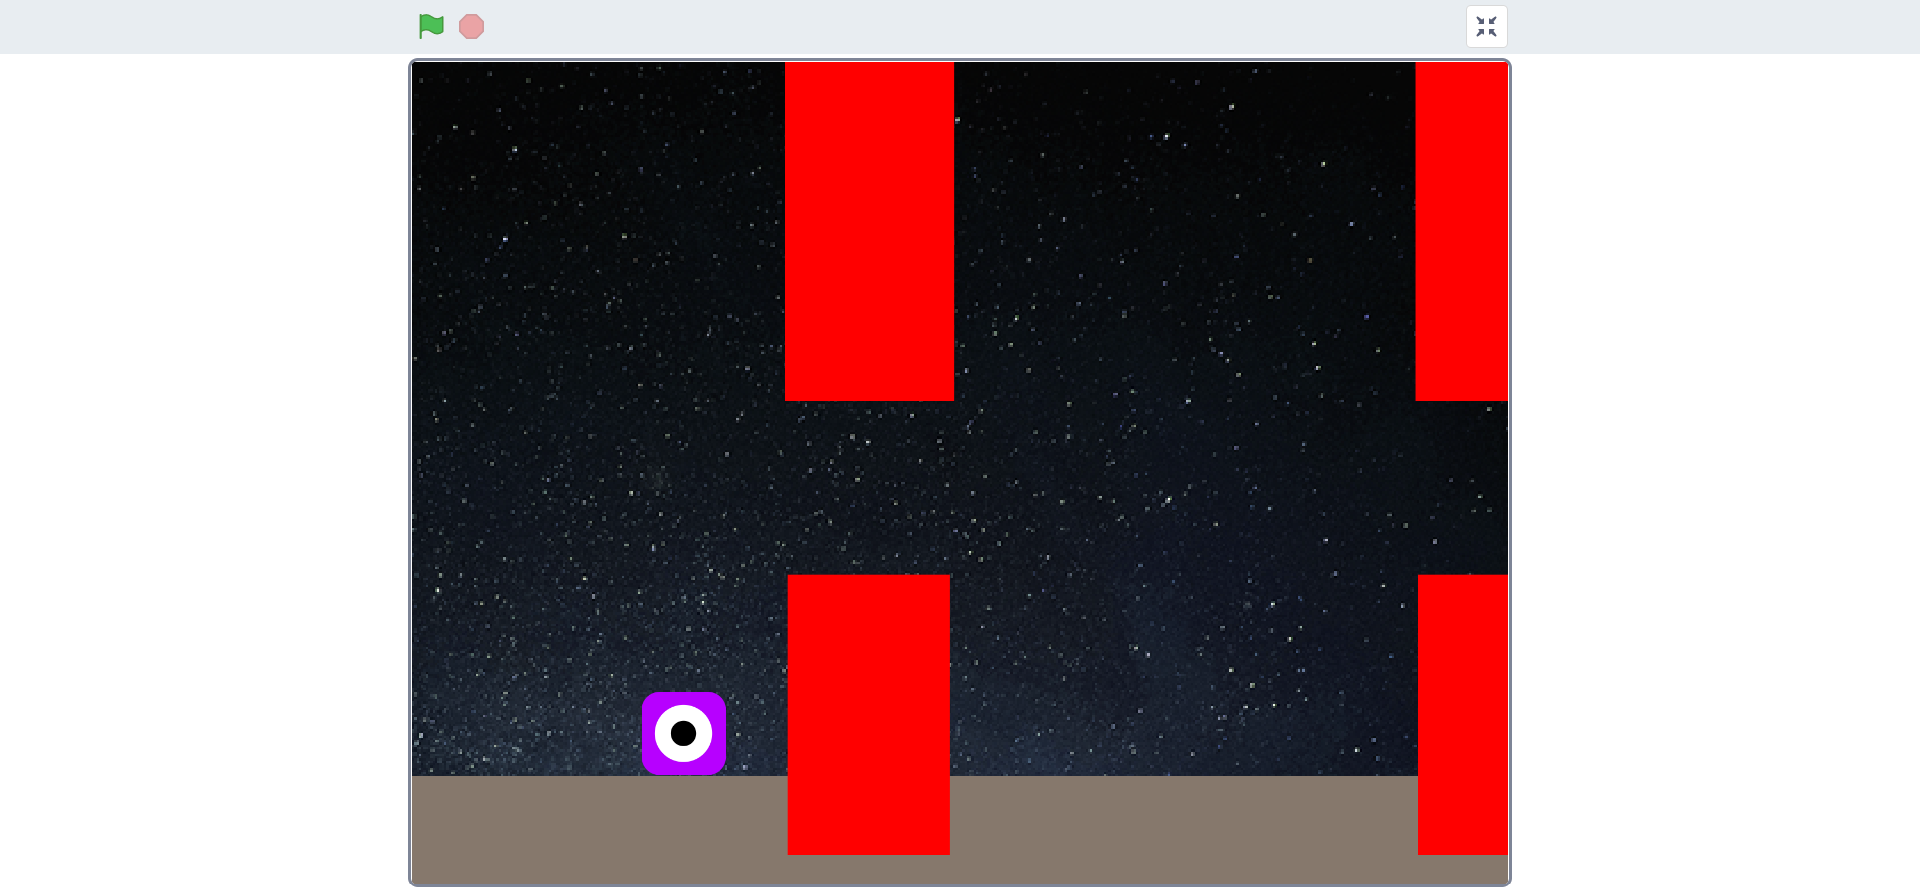
\includegraphics[width=1.0\linewidth,height=0.5\linewidth]{fig140001.png}
  \caption{Прескочи препятствията}
\label{fig140001}
\end{figure}

\section{Създаване на дизайна}
Първата стъпка от създаването на играта ще бъде добавянето на подходящи герои и фон. За героят на играта може да изберете от готовите герои в Scrach. Друг вариант е да го нарисувате, за да може играта ви да бъде по- интересна. Използвайки инструментите за рисуване може да създадете вашия герой (Фиг. \ref{fig140002}). В този проект ще демонстрира как да се създаде ефект, когато героят се движи. За тази цел трябва да бъде добавен още един костюм към него.

\begin{figure}[H]
  \centering
  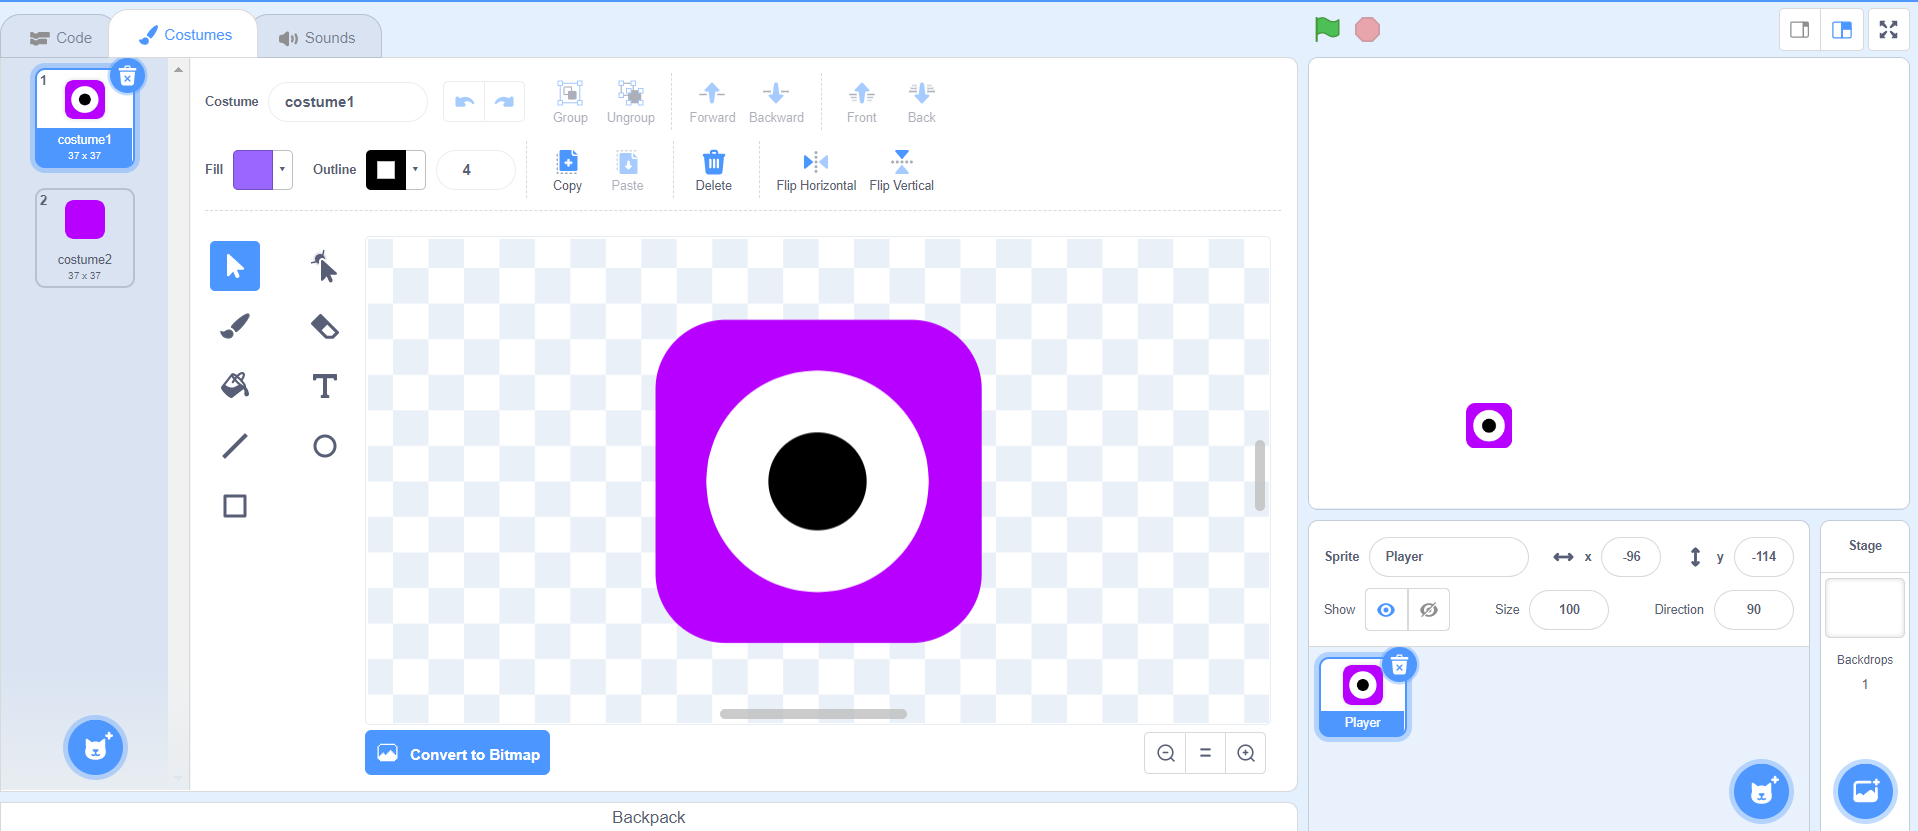
\includegraphics[width=1.0\linewidth,height=0.5\linewidth]{fig140002.png}
  \caption{Добавяне на основния герой}
\label{fig140002}
\end{figure}

В играта ще има нужда от един герой, който да е в долната част на трасето. Това е помощен герой, който ще служи за ориентир. Целта на лилавият герой е да се движи по него. Създайте го с помощта на инструментите за рисуване.

\begin{figure}[H]
  \centering
  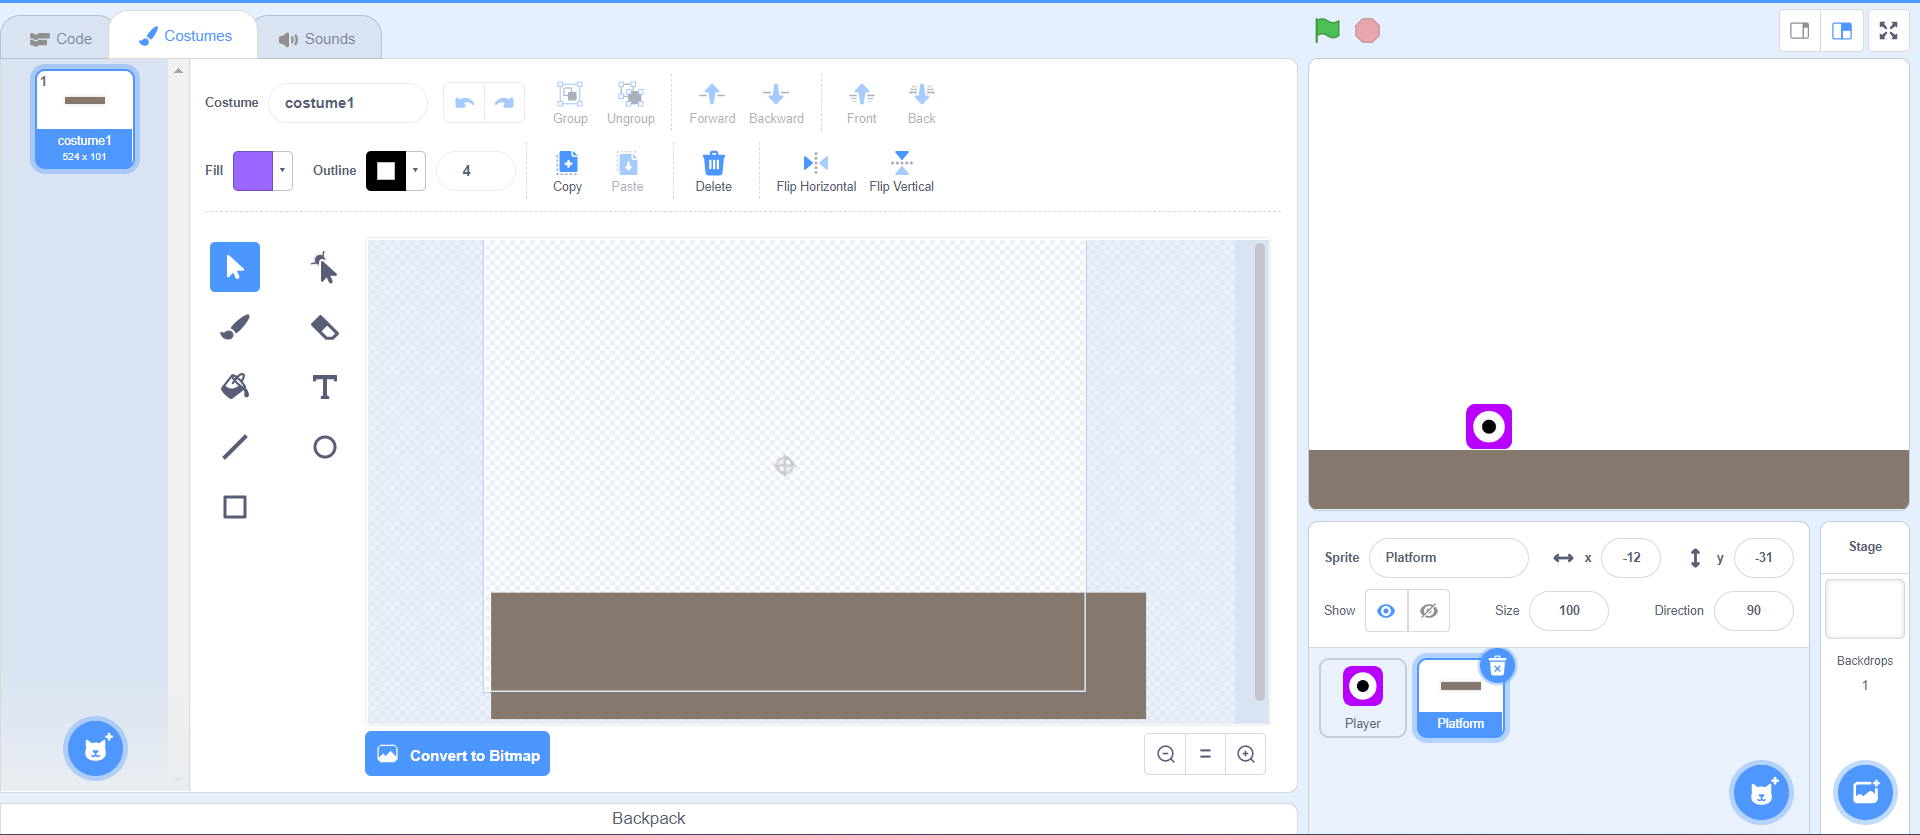
\includegraphics[width=1.0\linewidth,height=0.5\linewidth]{fig140003.png}
  \caption{Добавяне на помощния герой}
\label{fig140003}
\end{figure}

Последният герой който трябва да добавите е този за препятствията. Той отново трябва да бъде нарисуван с помощните инструменти. За да имате повече нива в играта, добавете повече костюми на героят ви. Когато лилавият ви герой премине през трасето, т.е. достигне до най-дясната точка на екрана, то тогава този герой ще си сменя костюма, която означава, че играчът ще премине на второ ниво.

\begin{figure}[H]
  \centering
  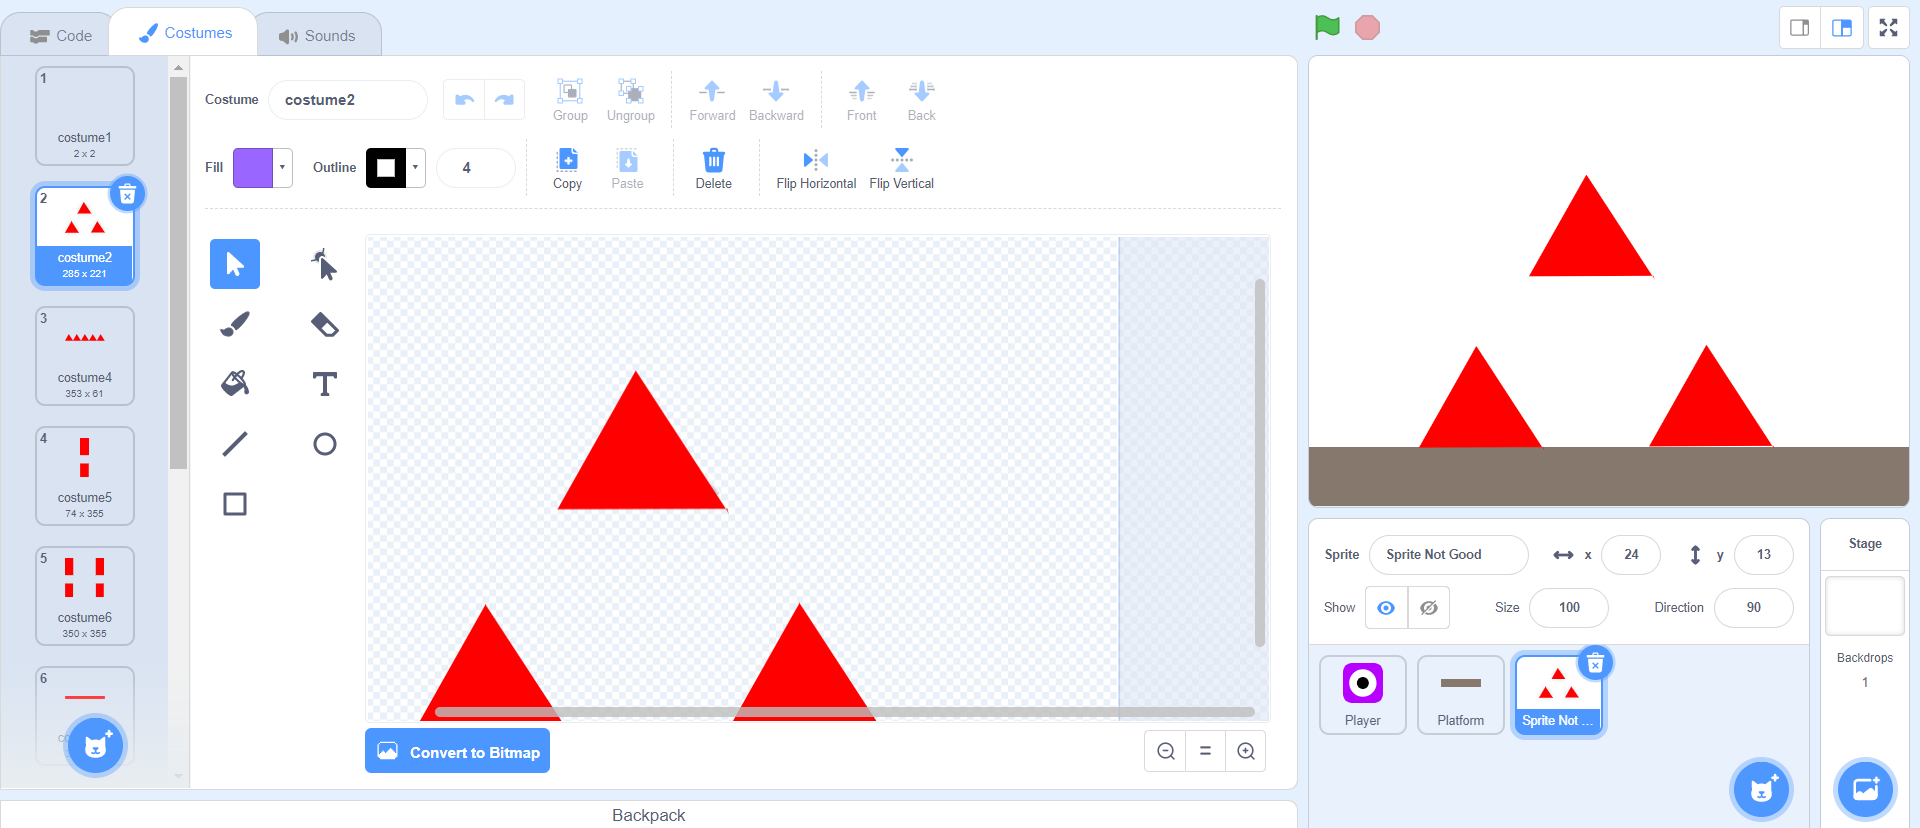
\includegraphics[width=1.0\linewidth,height=0.5\linewidth]{fig140004.png}
  \caption{Добавяне на препятствия}
\label{fig140004}
\end{figure}

За да ви бъде по- атрактивна играта добавете и подходящ фон. Също, както героите може да го изберете от вече готовите в Scratch или да си го нарисувате с помощта на инструментите.

\begin{figure}[H]
  \centering
  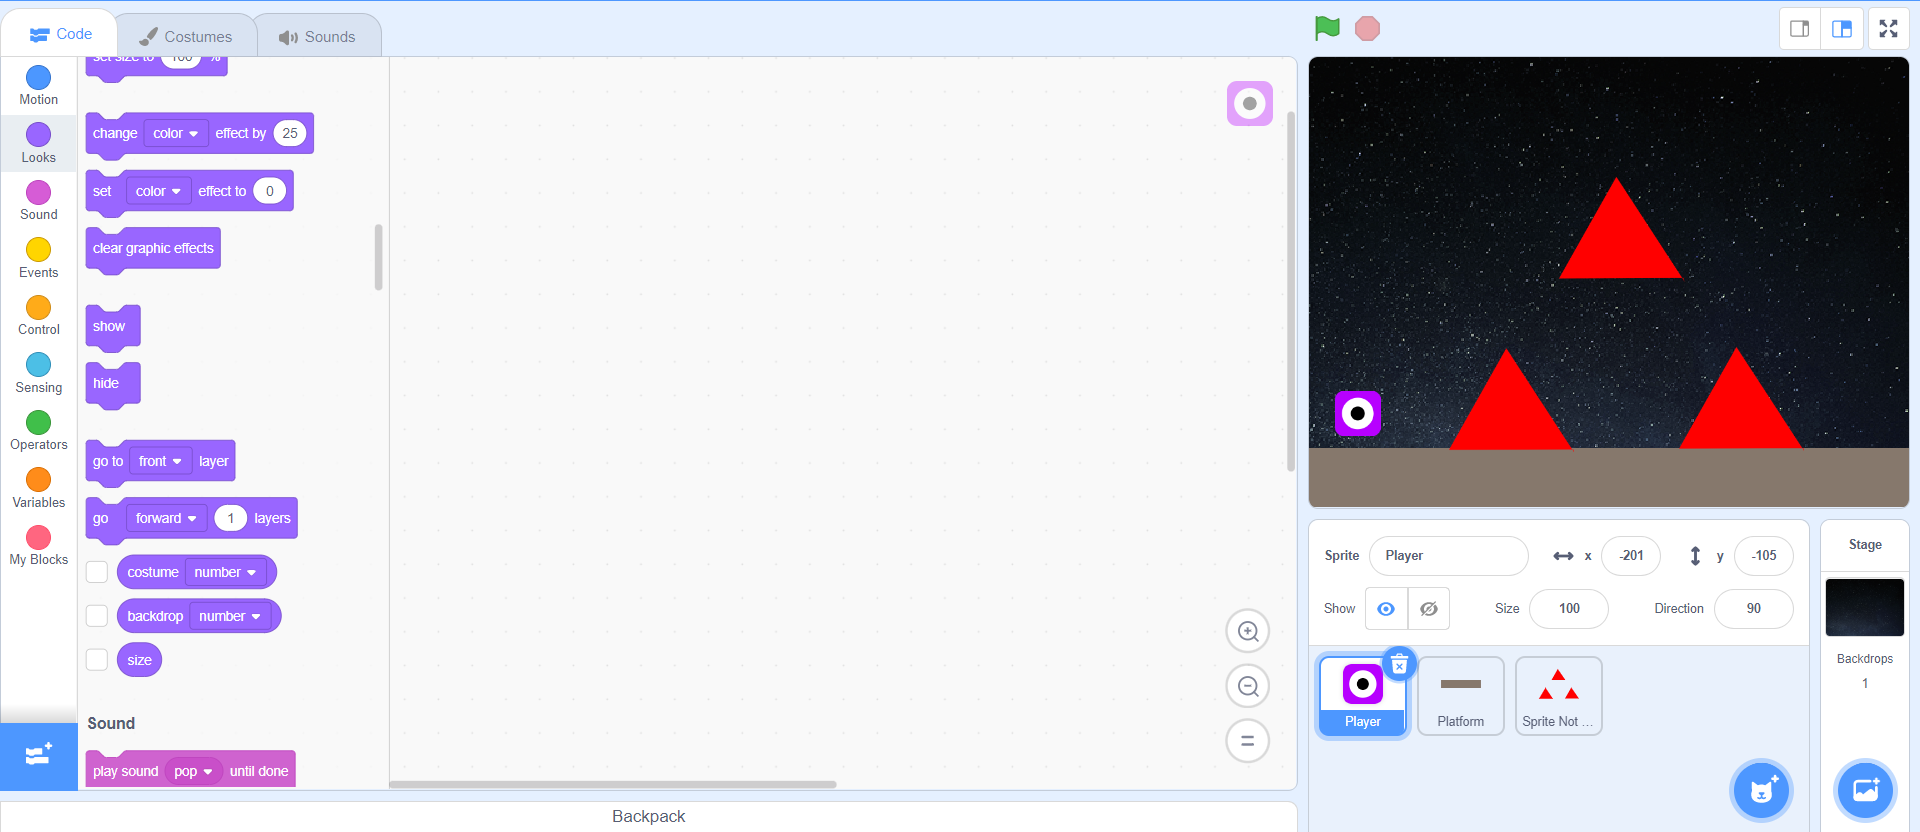
\includegraphics[width=1.0\linewidth,height=0.5\linewidth]{fig140005.png}
  \caption{Добавяне на фон}
\label{fig140005}
\end{figure}

\section{Програмиране на движението на героя}

Основният код, който трябва да добавите се намира в героят, който ще управлявате, в този случай лилавия герой. В тази игра ще имате нужда от 3 променливи - скорост на движение по оста x (xVel), скорост на движение по оста y (yVel) и скок (jump). От секция Variables изберете опцията Make a Variable и добавете променливите със съответните имена. За да не се показват по време на игра, може да махнете техните тикчета.

\begin{figure}[H]
  \centering
  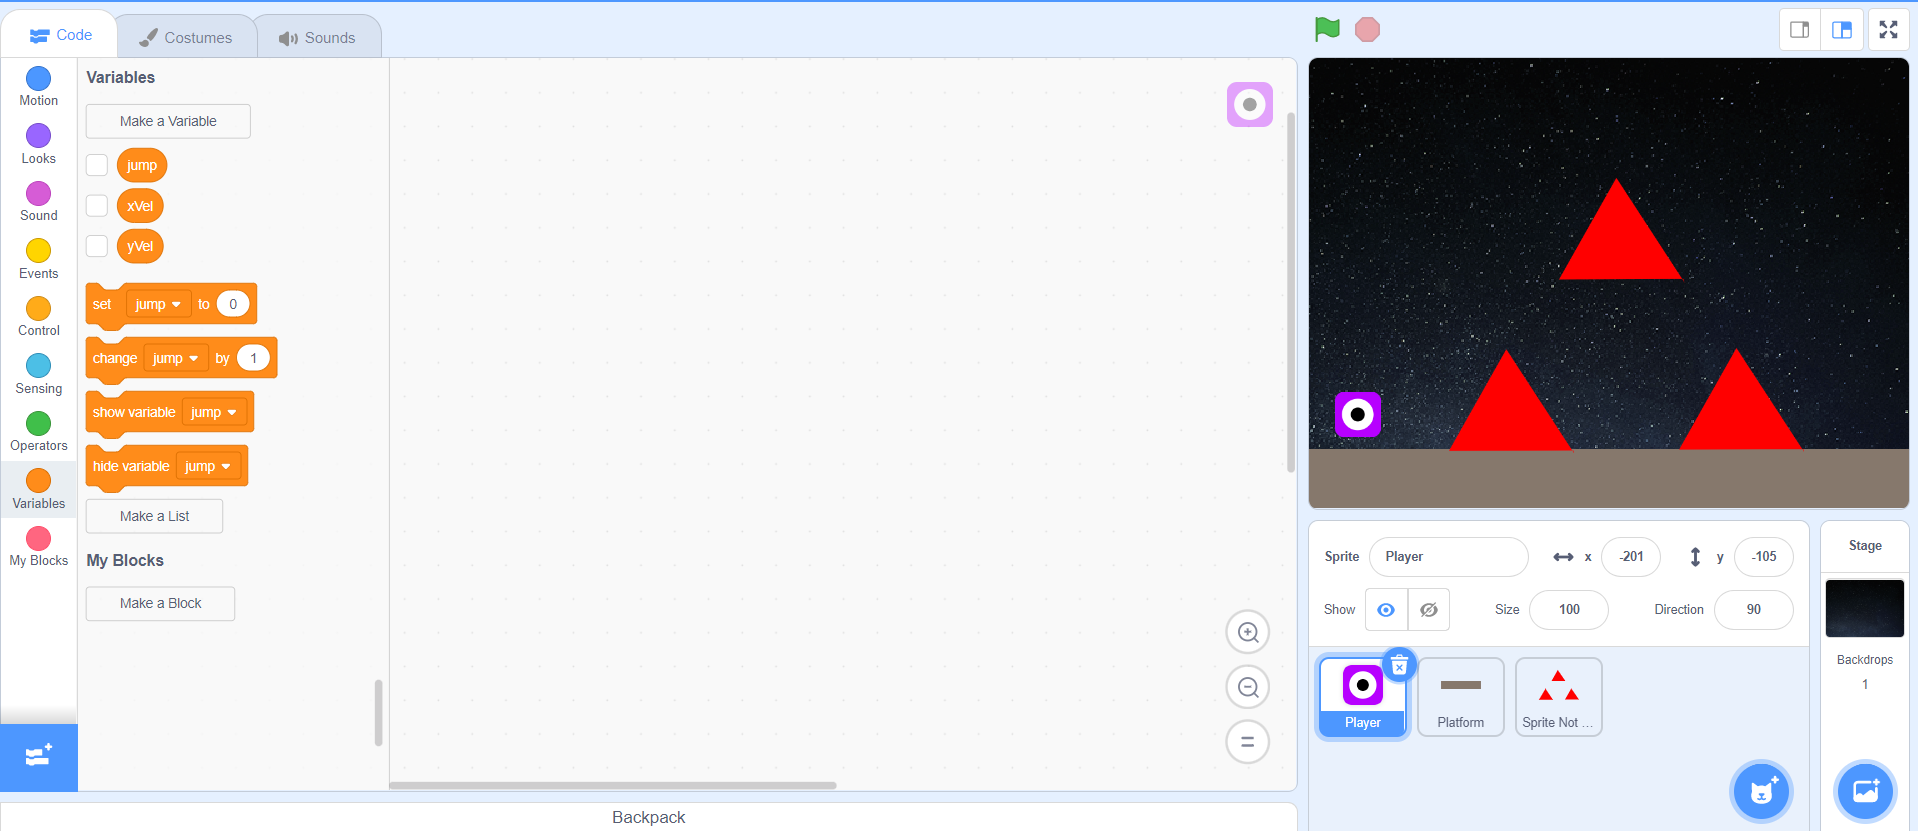
\includegraphics[width=1.0\linewidth,height=0.5\linewidth]{fig140006.png}
  \caption{Добавяне на променливите}
\label{fig140006}
\end{figure}

В началото на играта Стойността на тези променливи трябва да бъде равна на 0. За да бъде по- интересна играта позицията на героя ще бъде в средната част на екрана. Когато играта започне той ще се спусне надолу до платформата.

\begin{figure}[H]
  \centering
  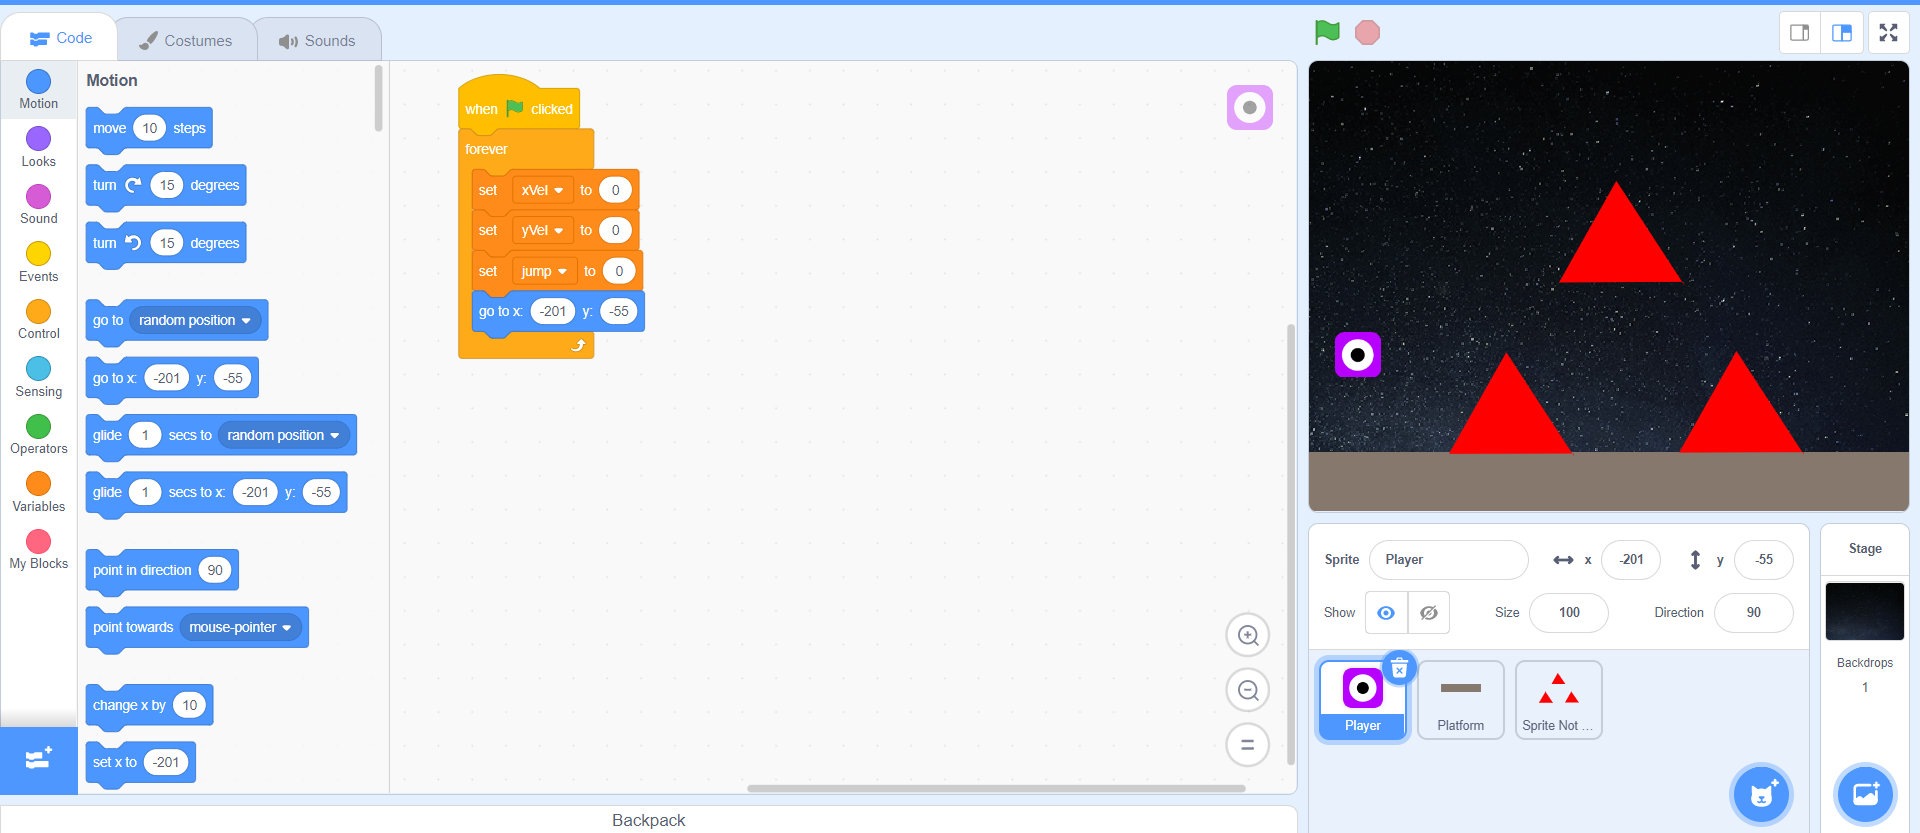
\includegraphics[width=1.0\linewidth,height=0.5\linewidth]{fig140007.png}
  \caption{Инициализиране на променливите}
\label{fig140007}
\end{figure}

Героят трябва да се движи докато не достигне до дясната част на екрана или докато не докосне героят препятствие. За тази цел първата инструкция, която трябва да добавите е repeat until блок. Условията, които трябва да добавите са две, които са разделени с операторът ИЛИ. Първото условие е x позицията на героя да бъде по- голяма от 240, което е краят на екрана. Второто условие е да докосва червеният герой.

\begin{figure}[H]
  \centering
  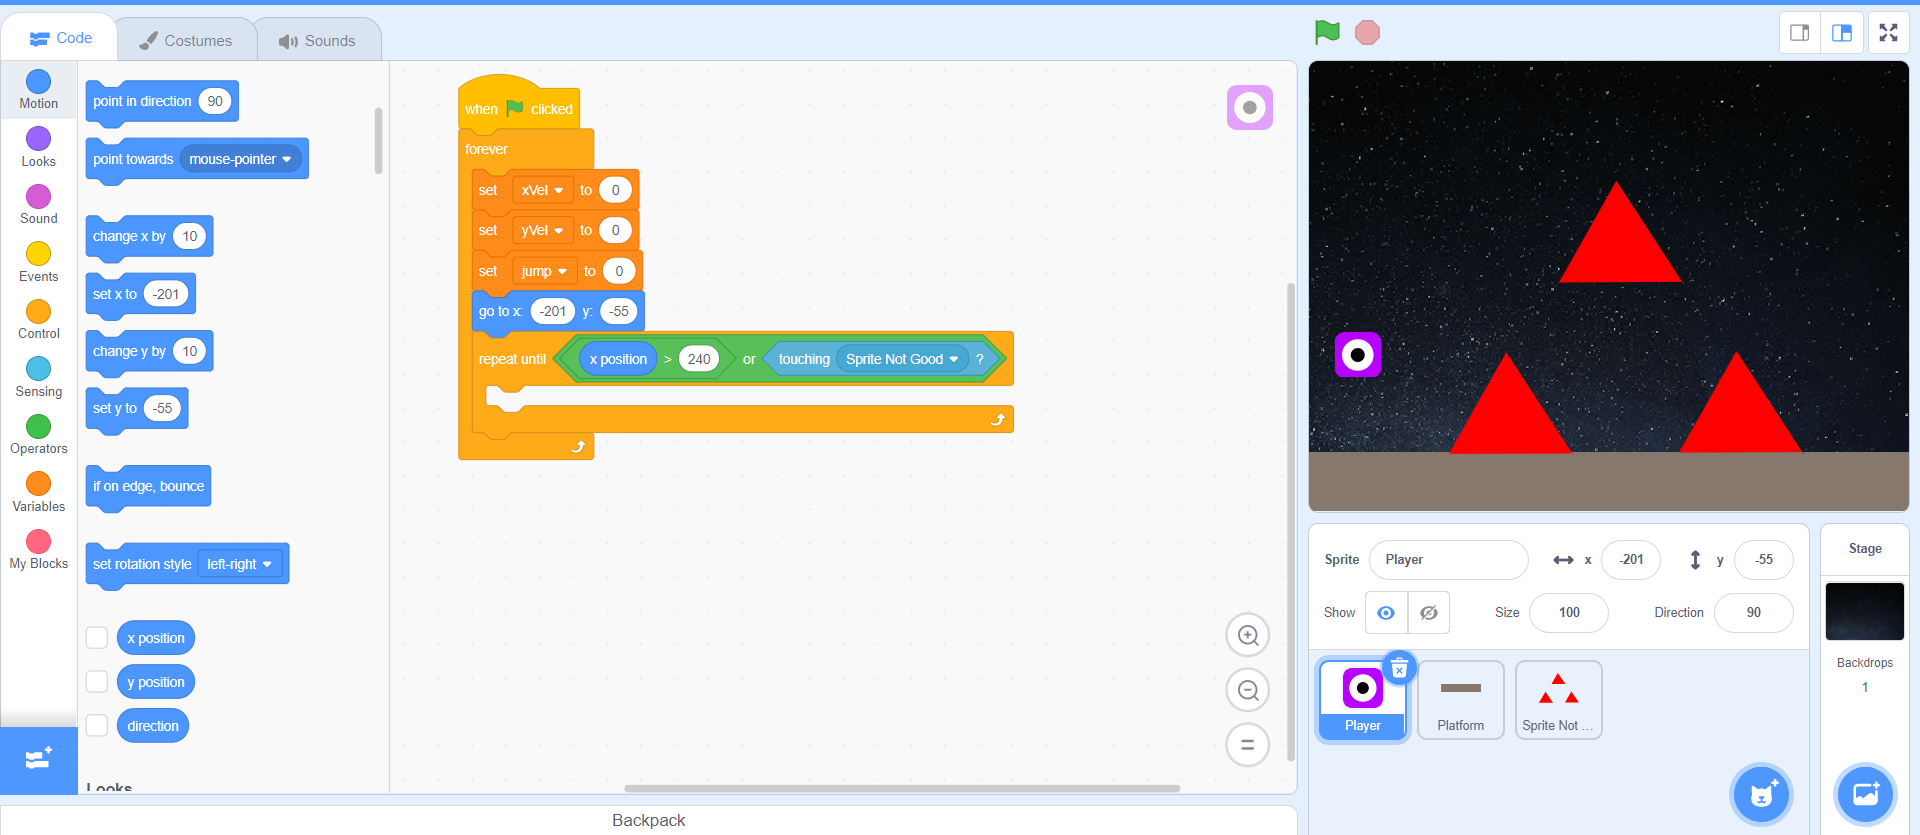
\includegraphics[width=1.0\linewidth,height=0.5\linewidth]{fig140008.png}
  \caption{Цикъл с условие за движение на героя}
\label{fig140008}
\end{figure}

За да се движи героят наляво и надясно ще използвате променливата xVel. От секцията за променливите е нужна инструкцията change xVel by. От секцията с операторите изберете този за изваждане. От едната страна сложете инструкцията за key right arrow pressed, а от дясната стрелка key left arrow pressed. Тази инструкция ще зададе стойност на променливата. Остава само да добавите инструкцията change x by и да поставите променливата. Така ако стартирате играта, героят ще се движи много бързо наляво и надясно. За това добавете инструкцията set xVel to xVel * 0.9. Стартирайте играта, за да тествате как героят се движи наляво и надясно.

\begin{figure}[H]
  \centering
  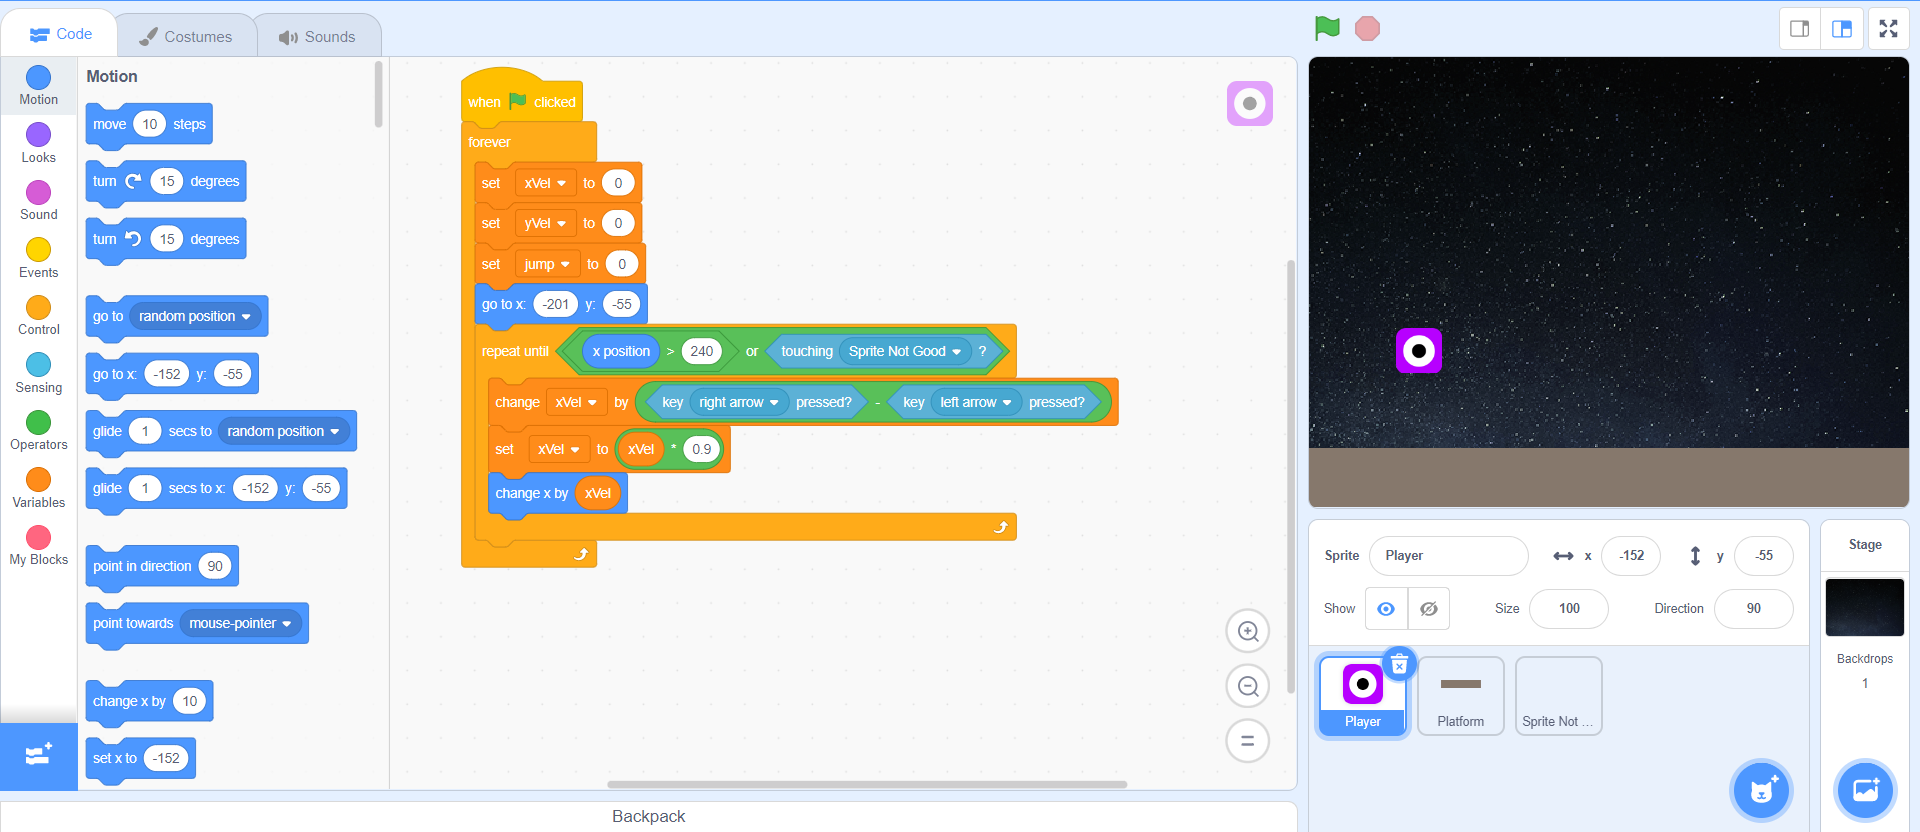
\includegraphics[width=1.0\linewidth,height=0.5\linewidth]{fig140009.png}
  \caption{Движение на героят наляво и надясно}
\label{fig140009}
\end{figure}

Следва да програмирате героят да подскача. В първата част ще програмирате, когато стартира играта или друго ниво героят от първоначалната позиция да слезе до платформата. За тази цел трябва да промените променливата yVel с -1 и да използвате инструкцията change y by със стойност променливата. Следва проверката ако докосва платформата. Ако условието е изпълнено, то тогава трябва да се сложи стойността на променливата yVel да бъде 0. Така единственият проблем ще е, че няма да спре да се движи героят, когато докосне платформата, защото главният цикъл ще се завърти още един път, защото неготово условие не е изпълнено. За това трябва да се промени позицията на y с yVel умножено по -1.

\begin{figure}[H]
  \centering
  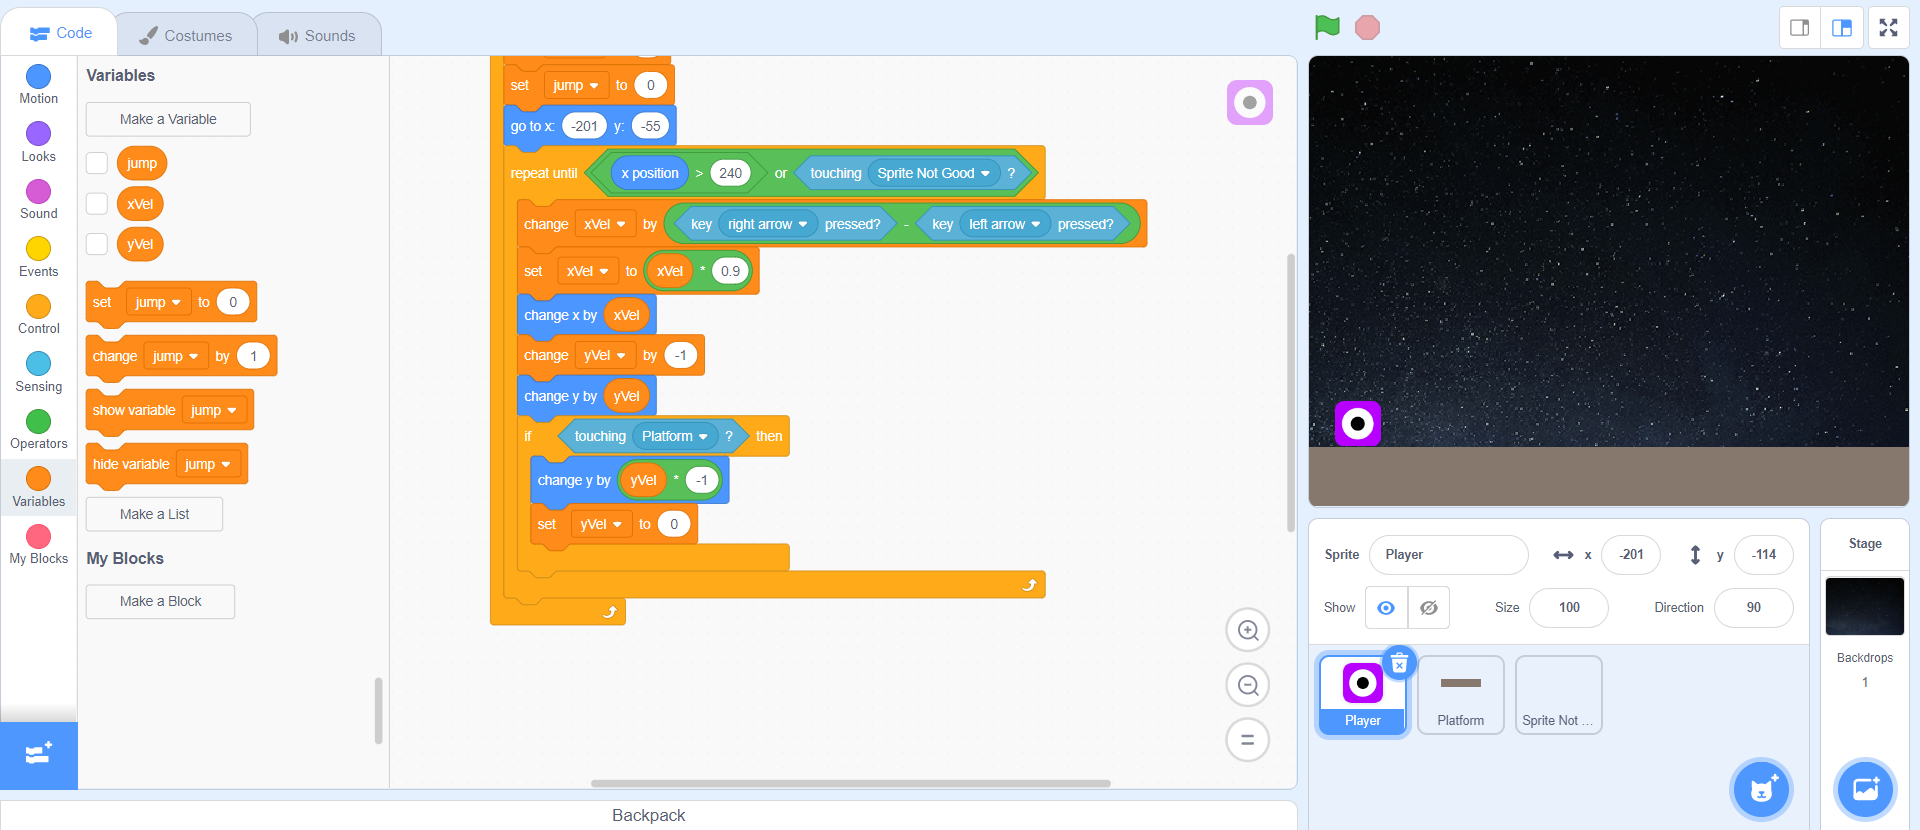
\includegraphics[width=1.0\linewidth,height=0.5\linewidth]{fig140010.png}
  \caption{Движение на героя надолу}
\label{fig140010}
\end{figure}

В последната част от създаването на алгоритъма за движението на лилавия герой ще бъде добавянето на подскоците. Ако играчът натисне стрелка нагоре, то променливата jump ще бъде равна на 1. Във всеки един от другите случаи тя трябва да бъде равна на 0, която означава, че героят няма да подскача. Първо трябва да добавите една проверка преди да направите стойността на yVel да бъде равна на 0. Тази проверка е трябва да проверява, ако yVel е по-малко от 0, то тогава героят не трябва да скача.

\begin{figure}[H]
  \centering
  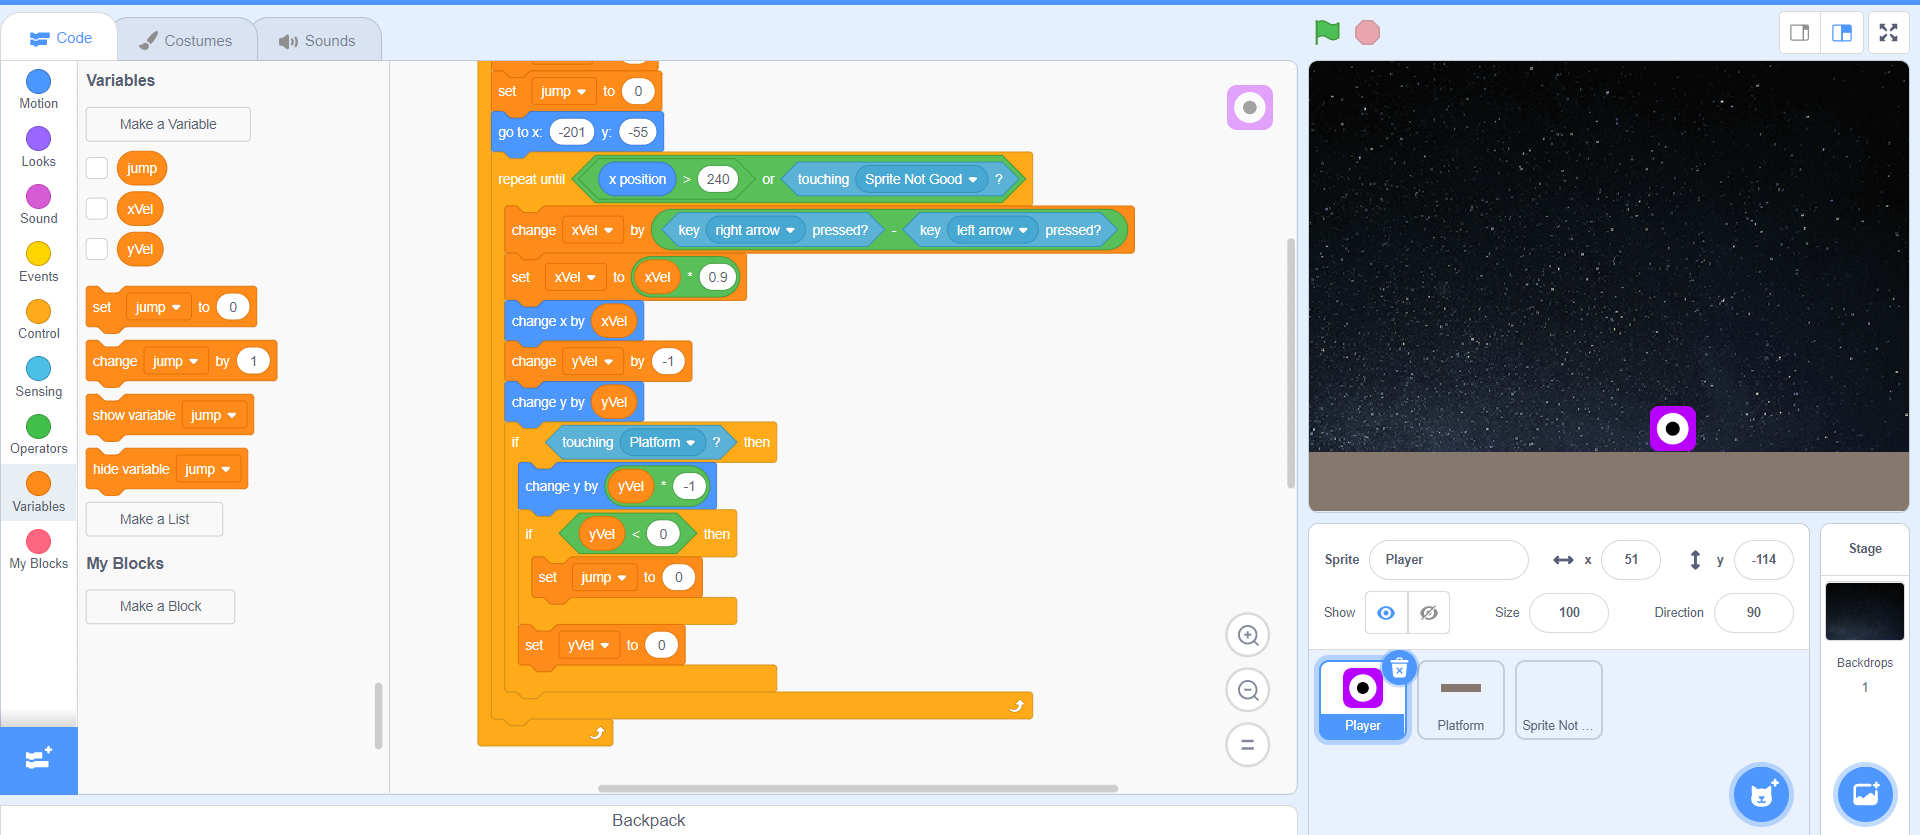
\includegraphics[width=1.0\linewidth,height=0.5\linewidth]{fig140011.png}
  \caption{Проверка, кога героят не скача}
\label{fig140011}
\end{figure}

Следва и проверка дали играчът е натиснал стрелка нагоре. Ако е и героят не подскача, то тогава трябва да се промени yVel с положително число и да се сложи променливата jump да е 1. Тествайте играта, за да видите как героят ви скача и се движи наляво и надясно.

\begin{figure}[H]
  \centering
  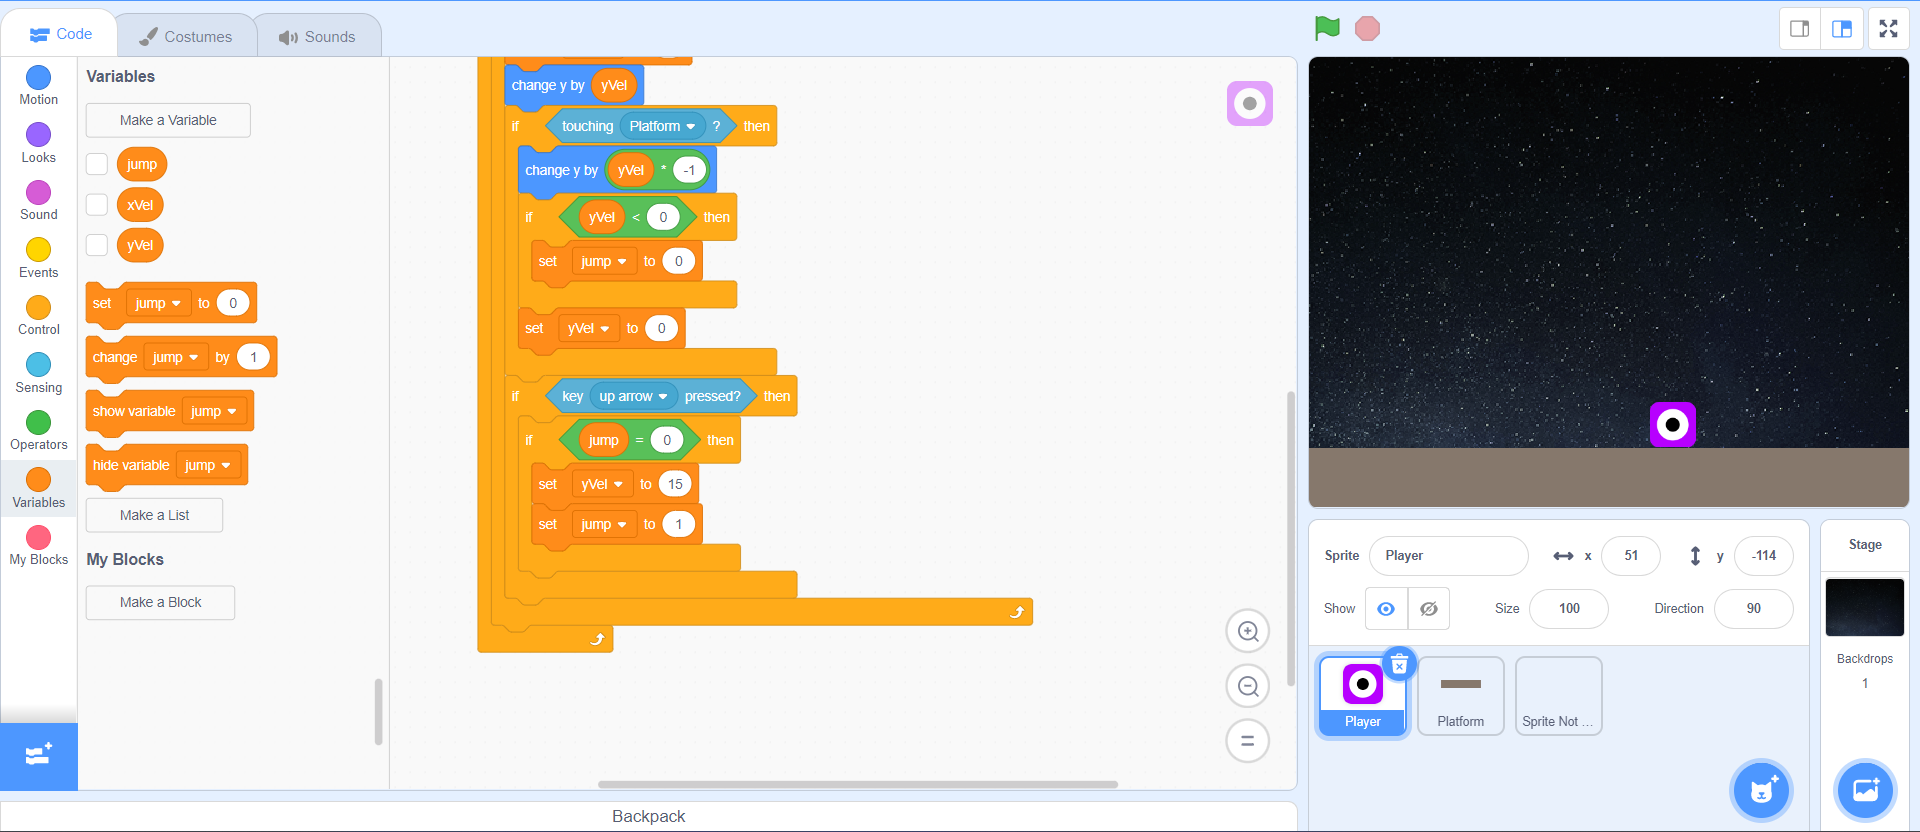
\includegraphics[width=1.0\linewidth,height=0.5\linewidth]{fig140012.png}
  \caption{Скок на героя при натискане на стрелка нагоре}
\label{fig140012}
\end{figure}

\section{Създаване на ефект, когато героят се движи}

След като сте приключили с движението на героя може да добавите и допълнителни инструкции, които да създават ефект, когато героят се движи. След проверката за натисната стрелка нагоре добавете инструкцията create clone of myself. Причината за това е, че ще бъде създаден клонинг на този герой, но с вторият му костюм. За това добавете нова инструкция, която е When I start as a clone. Тогава трябва да се смени костюма на героят, да бъде вторият му. Добавете цикъл, който да повтаря 10 пъти. Вътре в цикъла намалете размерите на героя клонинг и добавете прозрачен ефект. След цикъла изтрийте клонинга. Тествайте играта, за да видите какъв ефект се добави, когато се движите.

\begin{figure}[H]
  \centering
  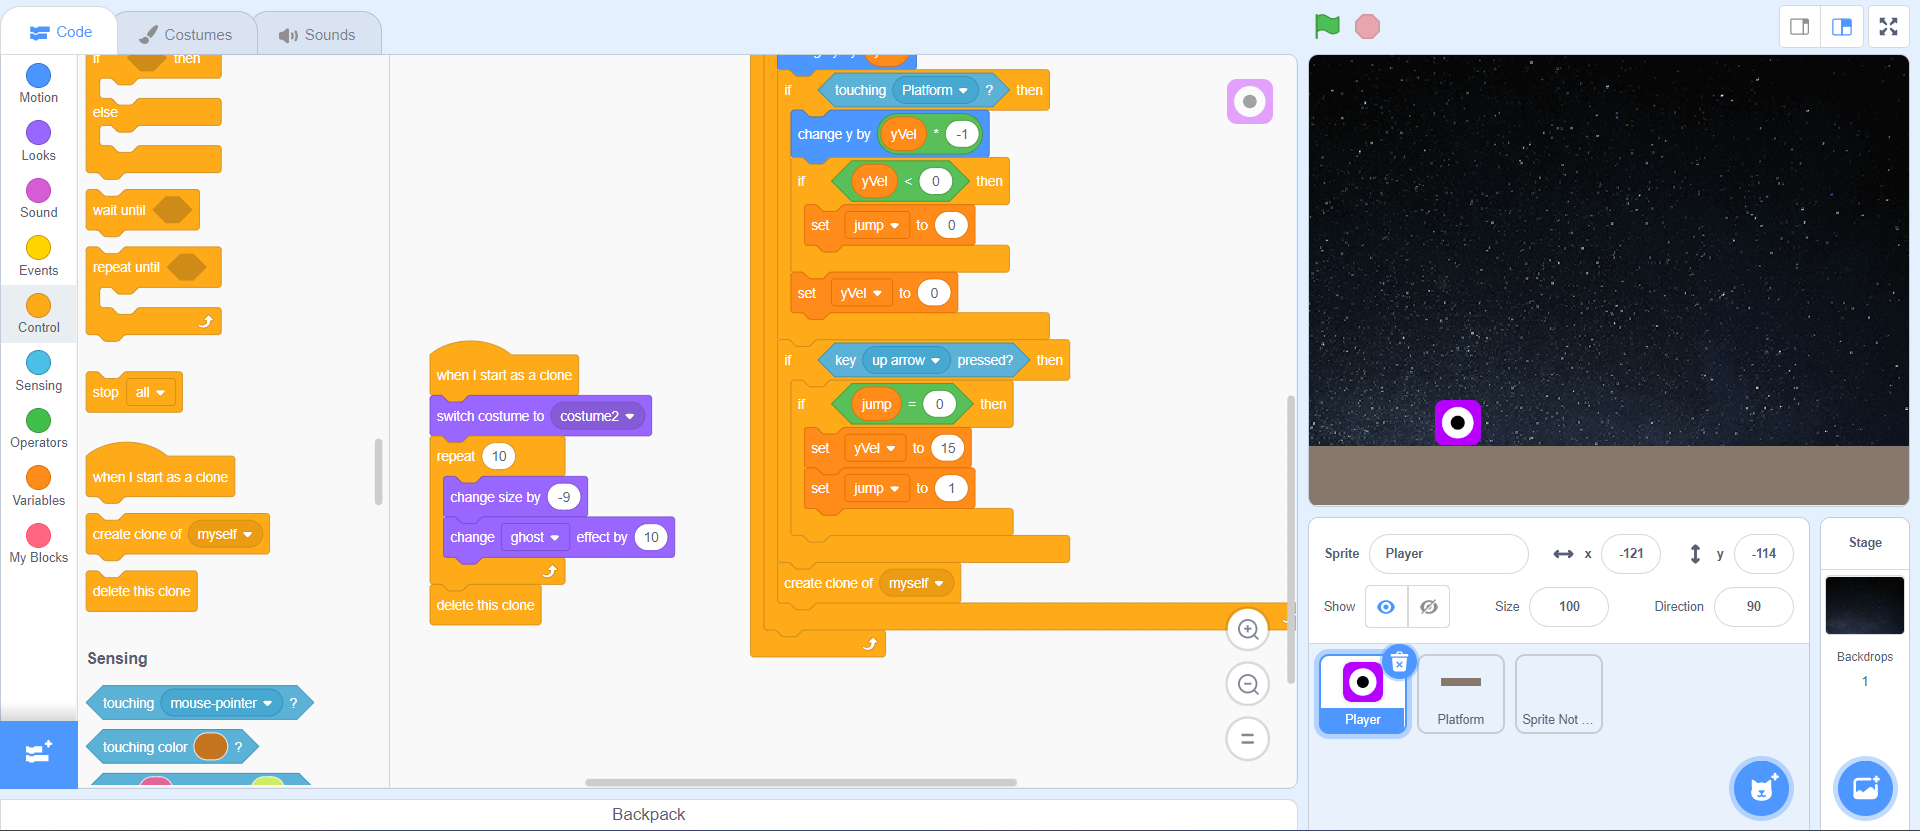
\includegraphics[width=1.0\linewidth,height=0.5\linewidth]{fig140013.png}
  \caption{Добавяне на ефект придвижване}
\label{fig140013}
\end{figure}

\section{Преминаване към следващо ниво}

В последната стъпка трябва да добавите инструкции героят да може да премине към следващо ниво. За тази цел в основният герой добавете проверката дали е достигнал до края на екрана. Ако е, то тогава нека да изпрати съобщение.

\begin{figure}[H]
  \centering
  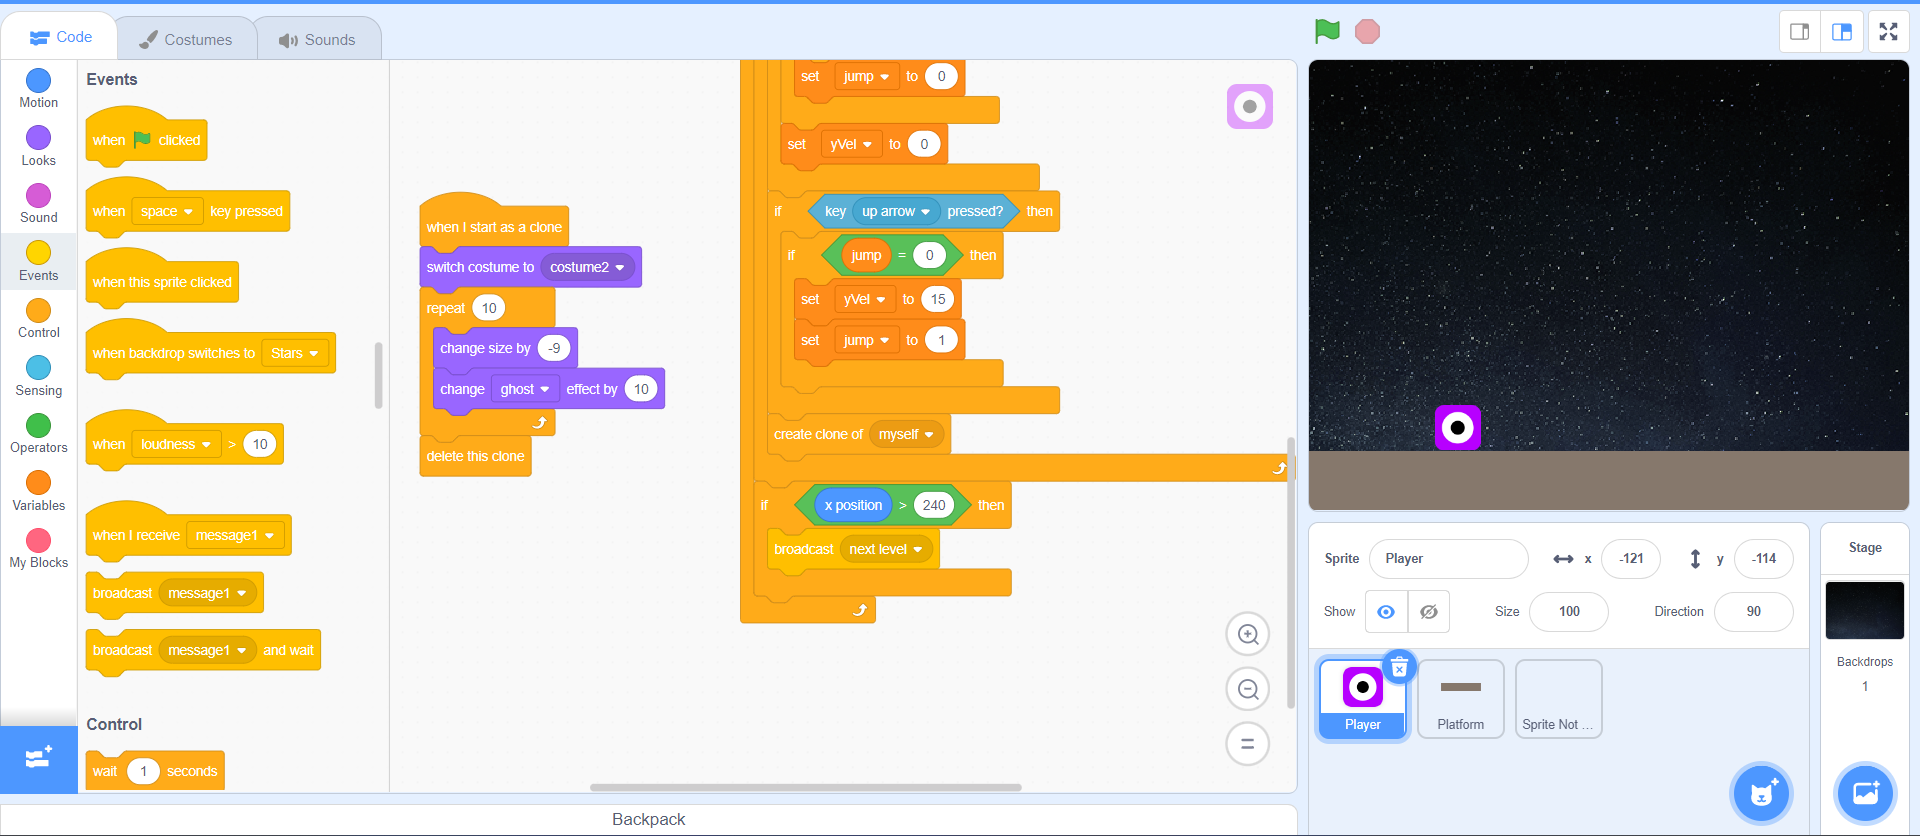
\includegraphics[width=1.0\linewidth,height=0.5\linewidth]{fig140014.png}
  \caption{Изпращане на съобщение за следващо ниво}
\label{fig140014}
\end{figure}

Изберете героят с червените препятствия. Добавете събитието, когато играта започне, тогава героят трябва да бъде с първоначалният си костюм. Добавете и второ събитие, когато получи съобщението за следващо ниво, то тогава трябва да смени костюма си. Стартирайте играта и се забавлявайте.

\begin{figure}[H]
  \centering
  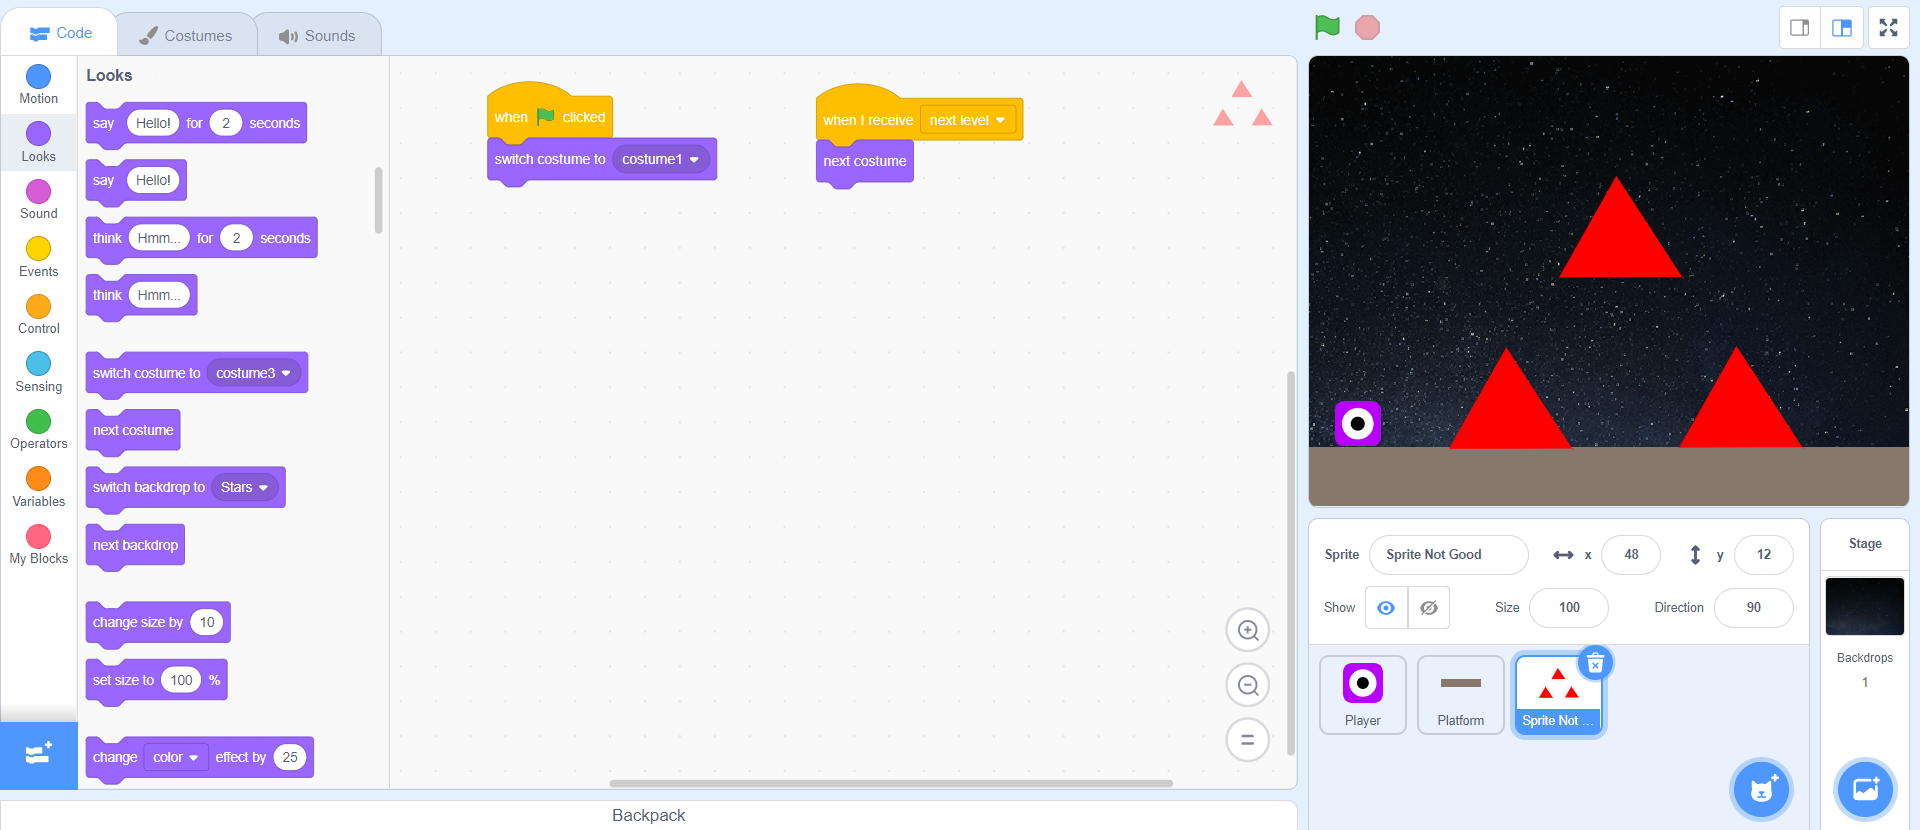
\includegraphics[width=1.0\linewidth,height=0.5\linewidth]{fig140015.png}
  \caption{Преминаване към следващо ниво}
\label{fig140015}
\end{figure}
